\section*{Analysis}
\label{analysis}

Det er valgt at analysere vores data med en \textbf{\textit{one-way repeated measures ANOVA}}. Hvor \textit{one-way} referere til antallet af uafhængige variabler, hvor vi har én, som er positionen af robotens hoved. 
Begrundelsen for at der laves en ANOVA er variablerne. Vi har én afhængig variabel som er vurderingen afgivet på skalaen, hvor typen af den indsamlede data er continuos. Vi har også kun én uafhængig variabel som er positionen af hovedet, hvor typen af data er fire kategorier, her er det antallet af kategorier der er årsag til valget af ANOVA, da der er flere end to. 
Analysen skal være \textit{repeated measures} da vi har et within-subjects design og derfor ønsker at sammenligne vurderinger fra samme testperson afgivet ved de forskellige positioner. 
\\\\
Før analysen udføres er der nogle antagelser som skal tjekkes om de er opfyldt. De er følgende: 
\begin{itemize}
	\item \textbf{Observationerne skal være uafhængige}\\
	?????? 
	\item \textbf{Den afhængige variabel skal som minimum være målt på en interval skala.}\\
	Vurderingen givet på skalaen er målt på en ratio skala og opfylder derved denne antagelse.
	\item \textbf{Der skal være homogen varians. }\\
	For at teste om der er homogen varians udføres Levene's test, hvor testresultatet er $F(3,28)=1,09, p=0,37$. Det viser at der ikke er signifikant forskel og det kan derfor konkluderes at antagelsen om homogen varians er opfyldt. 
	\item \textbf{Der skal være normalfordeling i grupperne.}\\
	For teste om der er normalfordeling udføres Shapiro-Wilk test, hvor resultatet er $W=0,94, p=0,09$. Heller ikke her er der signifikant forskel og det kan derfor konkluderes at antagelsen om normal fordeling er opfyldt.
\end{itemize}

\noindent Da alle antagelser for analysen er opfyldt, udføres denne i rstudio og giver resultatet: 
Der er signifikant effekt af positionen af robotens hoved på vurderingen af hvor indbydende den er, $F(3,21)=13,27, p=4,4*e^{-4}$

Analysen viser at der er en forskel, men ikke mellem hvilke positioner forskellen er. For at undersøge hvor forskellen er, udføres der post hoc test, mere specifikt den type der hedder \textit{pairwise comparisons using t-tests}. Resultatet af denne test kan ses i \autoref{fig:sammenligning}.
\begin{figure}[H]
\centering
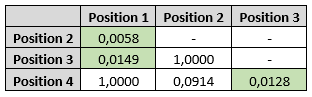
\includegraphics[width = 0.5\textwidth]{Figure/PostHocExcel.PNG} 
\caption{Sammenligning mellem vurderingerne afgivet til hver position. Grøn markering angiver at der er signifikant forskel.}
\label{fig:sammenligning}
\end{figure}

Resultatet viser at 